\section{STAR前向升级}

在过去二十余年的运行过程中,STAR采集了许多 质子-质子,质子-金对撞的数据,并且基于这些数据在cold QCD领域得到了很好的测量结果。STAR的主要探测器集中在中心赝快度区域($|\eta| < 1$),
有关前向的物理测量较少,但不论对于cold QCD还是重离子对撞来说,前向方向都是一个十分令人感兴趣的区间。有着丰富的物理目标等着我们去探索。

在过去的二十年当中,STAR前向的测量任务主要由前向介子谱仪(Forward Meson Spectrometer, FMS)完成。
前向介子谱仪是一个安装在STAR西侧前向快度区间的电磁量能器,其由两种不同规格共计1264块铅玻璃构成。如图\ref{fig:FMS}所示。前向介子谱仪是一个全吸收型电磁量能器,铅玻璃可以同时充当能量沉积的载体和探测手段。
但对于电磁量能器来说,其主要鉴别电子的手段是通过计算E/p 的值从而进行电子鉴别。这就要求除了单独的一个量能器我们还需要有能力对打在探测器上的粒子进行径迹和动量的探测,所以我们希望前向除了量能器以外能额外的有径迹探测的手段。并且作为电磁量能器,前向介子谱仪并不能对$\pi^0$、中子、光子等中性粒子进行测量。

在近些年来STAR实验进行了一些升级,例如前文提到的iTPC升级以及新加装的事例平面探测器(Event Plane Detector, EPC)。但iTPC作为STAR主径迹探测器时间投影室的一部分,覆盖的赝快度区间仍然有限,不能覆盖 $|\eta| > 2$的范围。而事例平面探测器虽然可以覆盖较为前向(西侧)和背向(东侧)的赝快度范围($2.14 < |\eta| < 5.09 $),但其探测器每个最小探测单元粒度很大,且只有一层,无法进行径迹重建。如果同时可以扩展径迹探测器所覆盖的赝快度区间,STAR实验将有能力对极大或者极小的Bjorken x区间进行更多物理量的测量,有助于加深对cold QCD的理解。同时RHIC将于2025年开始进行升级成为电子-离子对撞机(Electron-Ion Collider, EIC)。在前向的物理测量和探测器升级可以为以后基于电子-离子对撞机的探测器建设起指导作用和积累经验。

基于这些需求,STAR提出了前向升级计划(Forward Upgrade),如图\ref{fig:FWD}所示,覆盖了$ 2.5 < \eta < 4 $的赝快度区间。整个前向升级由两部分构成:前向量能器系统(Forward Calorimeter Systerm, FCS)和前向径迹探测系统(Forward Tracking System, FTS)。其中前向量能器系统由电磁量能器(Electromagnetic Calorimeter, Ecal)和强子量能器(Hadronic Calorimeter, HCal)组成。前向电磁量能器为铅闪烁体取样量能器,前向强子量能器为三明治型铁闪烁体板取样型量能器。前向电磁量能器和强子量能器都有着很好的能量分辨,电磁量能器能量分辨可达到~$8\%/\sqrt{E}$,强子量能器的能量分辨可以达到~$70\%/\sqrt{E}$。
\begin{figure}[htb]
    \begin{center}
    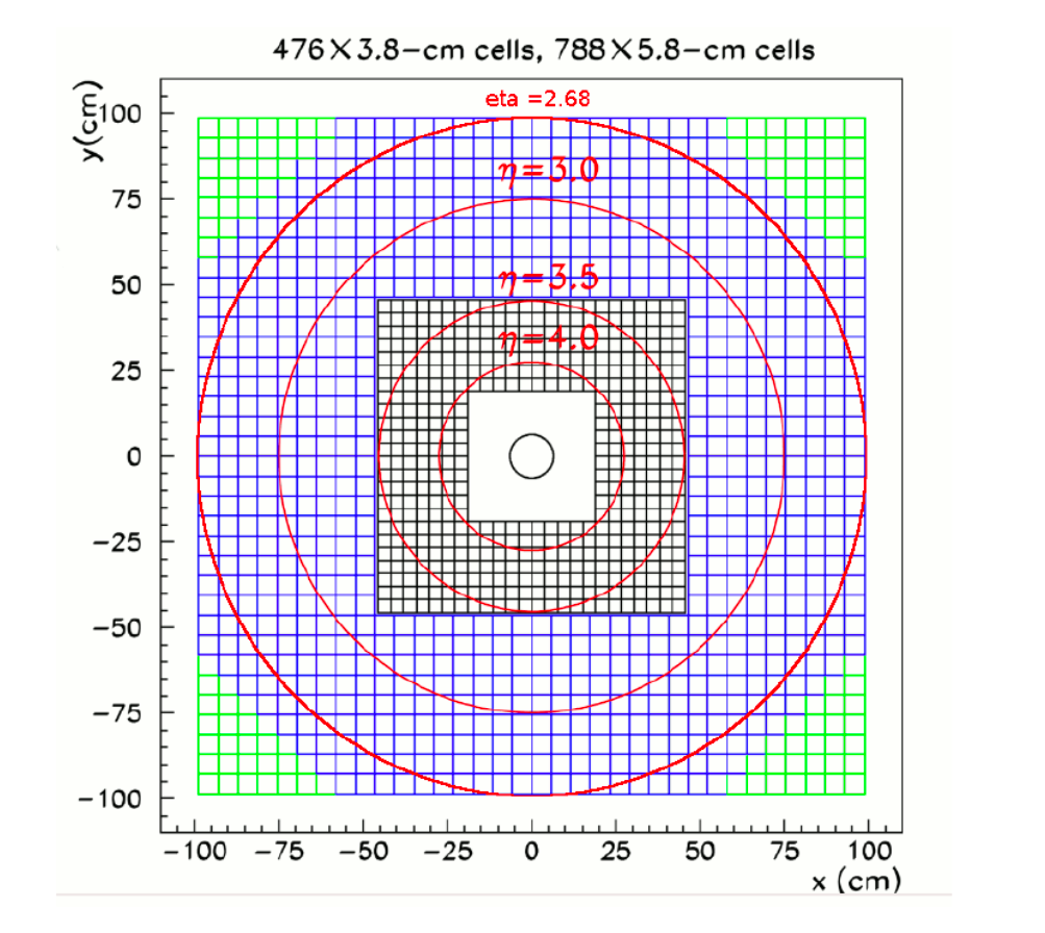
\includegraphics[width=0.8\textwidth,clip]{figures/Chapter3/FMS.png}
    \end{center}
    \caption[前向介子谱仪(FMS)示意图]{前向介子谱仪(FMS)示意图}
    \label{fig:FMS}
\end{figure}
\begin{figure}[htb]
    \begin{center}
    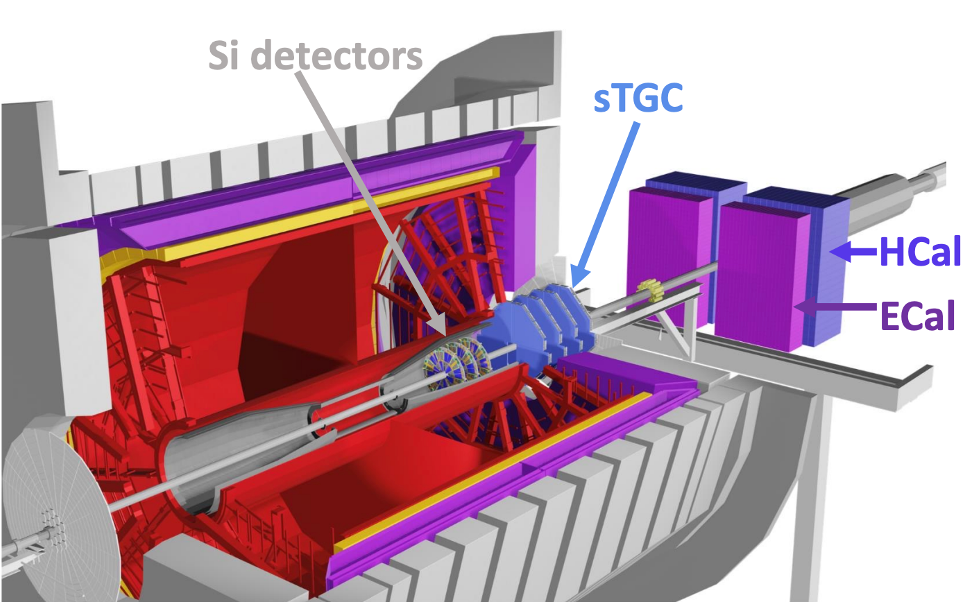
\includegraphics[width=0.8\textwidth,clip]{figures/Chapter3/FWD.png}
    \end{center}
    \caption[STAR前向升级示意图]{STAR前向升级示意图,各子探测器已在图上标出}
    \label{fig:FWD}
\end{figure}
前向硅径迹探测器(Forward Silicon Tracker, FST)和前向窄气隙室径迹探测器(Forward sTGC Tracker, FTT)共同组成了STAR前向升级当中的前向径迹探测系统。

因为STAR在Run14-Run16期间曾经在对撞点(Interaction point)附近安装过重味粒子径迹探测器(Heavy Flavor Tracker, HFT),有过硅径迹探测器的安装操作经验,所以硅探测器被考虑用来作为前向径迹探测器的一部分。前向硅径迹探测器由三层圆盘状的硅探测器组成,覆盖$2\pi$的方位角和$2.5 < \eta < 4$的快度区间。作为径迹探测系统的一部分,前向硅径迹探测器可以为整个径迹系统提供三个点来进行径迹重建。

在过去的二十年间,窄隙室得到了长足的发展并被应用到了ATLAS实验前向New Small Wheel升级当中,技术已经相对成熟,有着成本低和物质的量小的优点,适合在离对撞点较远的位置用于径迹探测。整个前向窄气隙室径迹探测器由四层sTGC平面组成,可以为径迹探测系统提供四个点用于径迹重建。对于每一个sTGC平面,其由四个五边形的模块拼接而成,如图 \ref{fig:sTGC} 所示。
\begin{figure}[htb]
    \begin{center}
    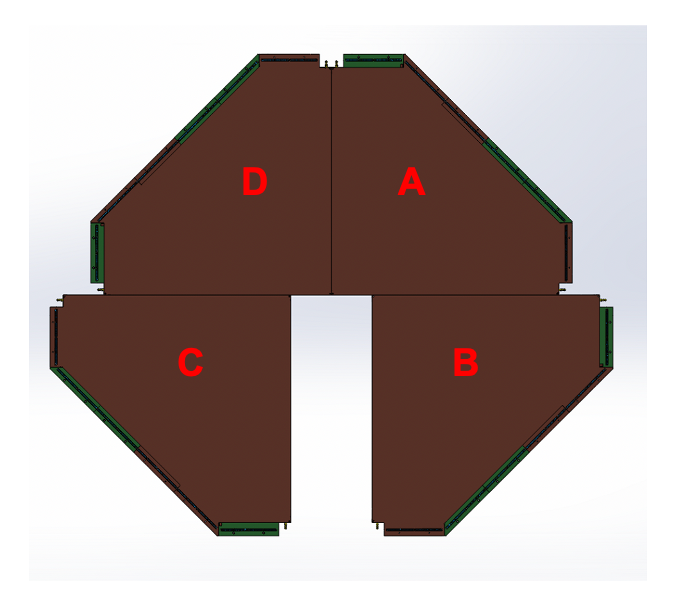
\includegraphics[width=0.7\textwidth,clip]{figures/Chapter2/sTGC.png}
    \end{center}
    \caption[前向小气隙室径迹探测器单个平面正视图]{前向小气隙室径迹探测器单个平面正视图,每个平面由四个五边形sTGC模块组成。}
    \label{fig:sTGC}
\end{figure}

笔者在攻读博士学位期间参与了sTGC在布鲁克海文国家实验室的测试以及cluster finder编写工作,将在接下来的几个小节中对窄隙室以及笔者的工作进行详细介绍。